\documentclass[a4paper,12pt]{article}

\usepackage[utf8x]{inputenc}
\usepackage[T2A]{fontenc}
\usepackage[english, russian]{babel}

% Опционно, требует  apt-get install scalable-cyrfonts.*
% и удаления одной строчки в cyrtimes.sty
% Сточку не удалять!
% \usepackage{cyrtimes}

% Картнки и tikz
\usepackage{graphicx}
\usepackage{tikz}
\usetikzlibrary{snakes,arrows,shapes}


% Некоторая русификация.
\usepackage{misccorr}
\usepackage{indentfirst}
\renewcommand{\labelitemi}{\normalfont\bfseries{--}}

% Увы, поля придётся уменьшить из-за листингов.
\topmargin -1cm
\oddsidemargin -0.5cm
\evensidemargin -0.5cm
\textwidth 17cm
\textheight 24cm

\sloppy

% Оглавление в PDF
\usepackage[
bookmarks=true,
colorlinks=true, linkcolor=black, anchorcolor=black, citecolor=black, menucolor=black,filecolor=black, urlcolor=black,
unicode=true
]{hyperref}

% Для исходного кода в тексте
\newcommand{\Code}[1]{\texttt{#1}}

\usepackage{verbatim}
\usepackage{fancyvrb}
\fvset{frame=leftline, fontsize=\small, framerule=0.4mm, rulecolor=\color{darkgray}, commandchars=\\\{\}}
\renewcommand{\theFancyVerbLine}{\small\arabic{FancyVerbLine}}


\title{Отчёт по лабораторной работе \\ <<IP-маршрутизация>>}
\author{Пучнина Анастасия Ивановна}

\begin{document}

\maketitle

\tableofcontents

% Текст отчёта должен быть читаемым!!! Написанное здесь является рыбой.

\section{Топология сети}

Топология сети и использыемые IP-адреса показаны на рис.~\ref{fig:network}.

\begin{figure}
\centering
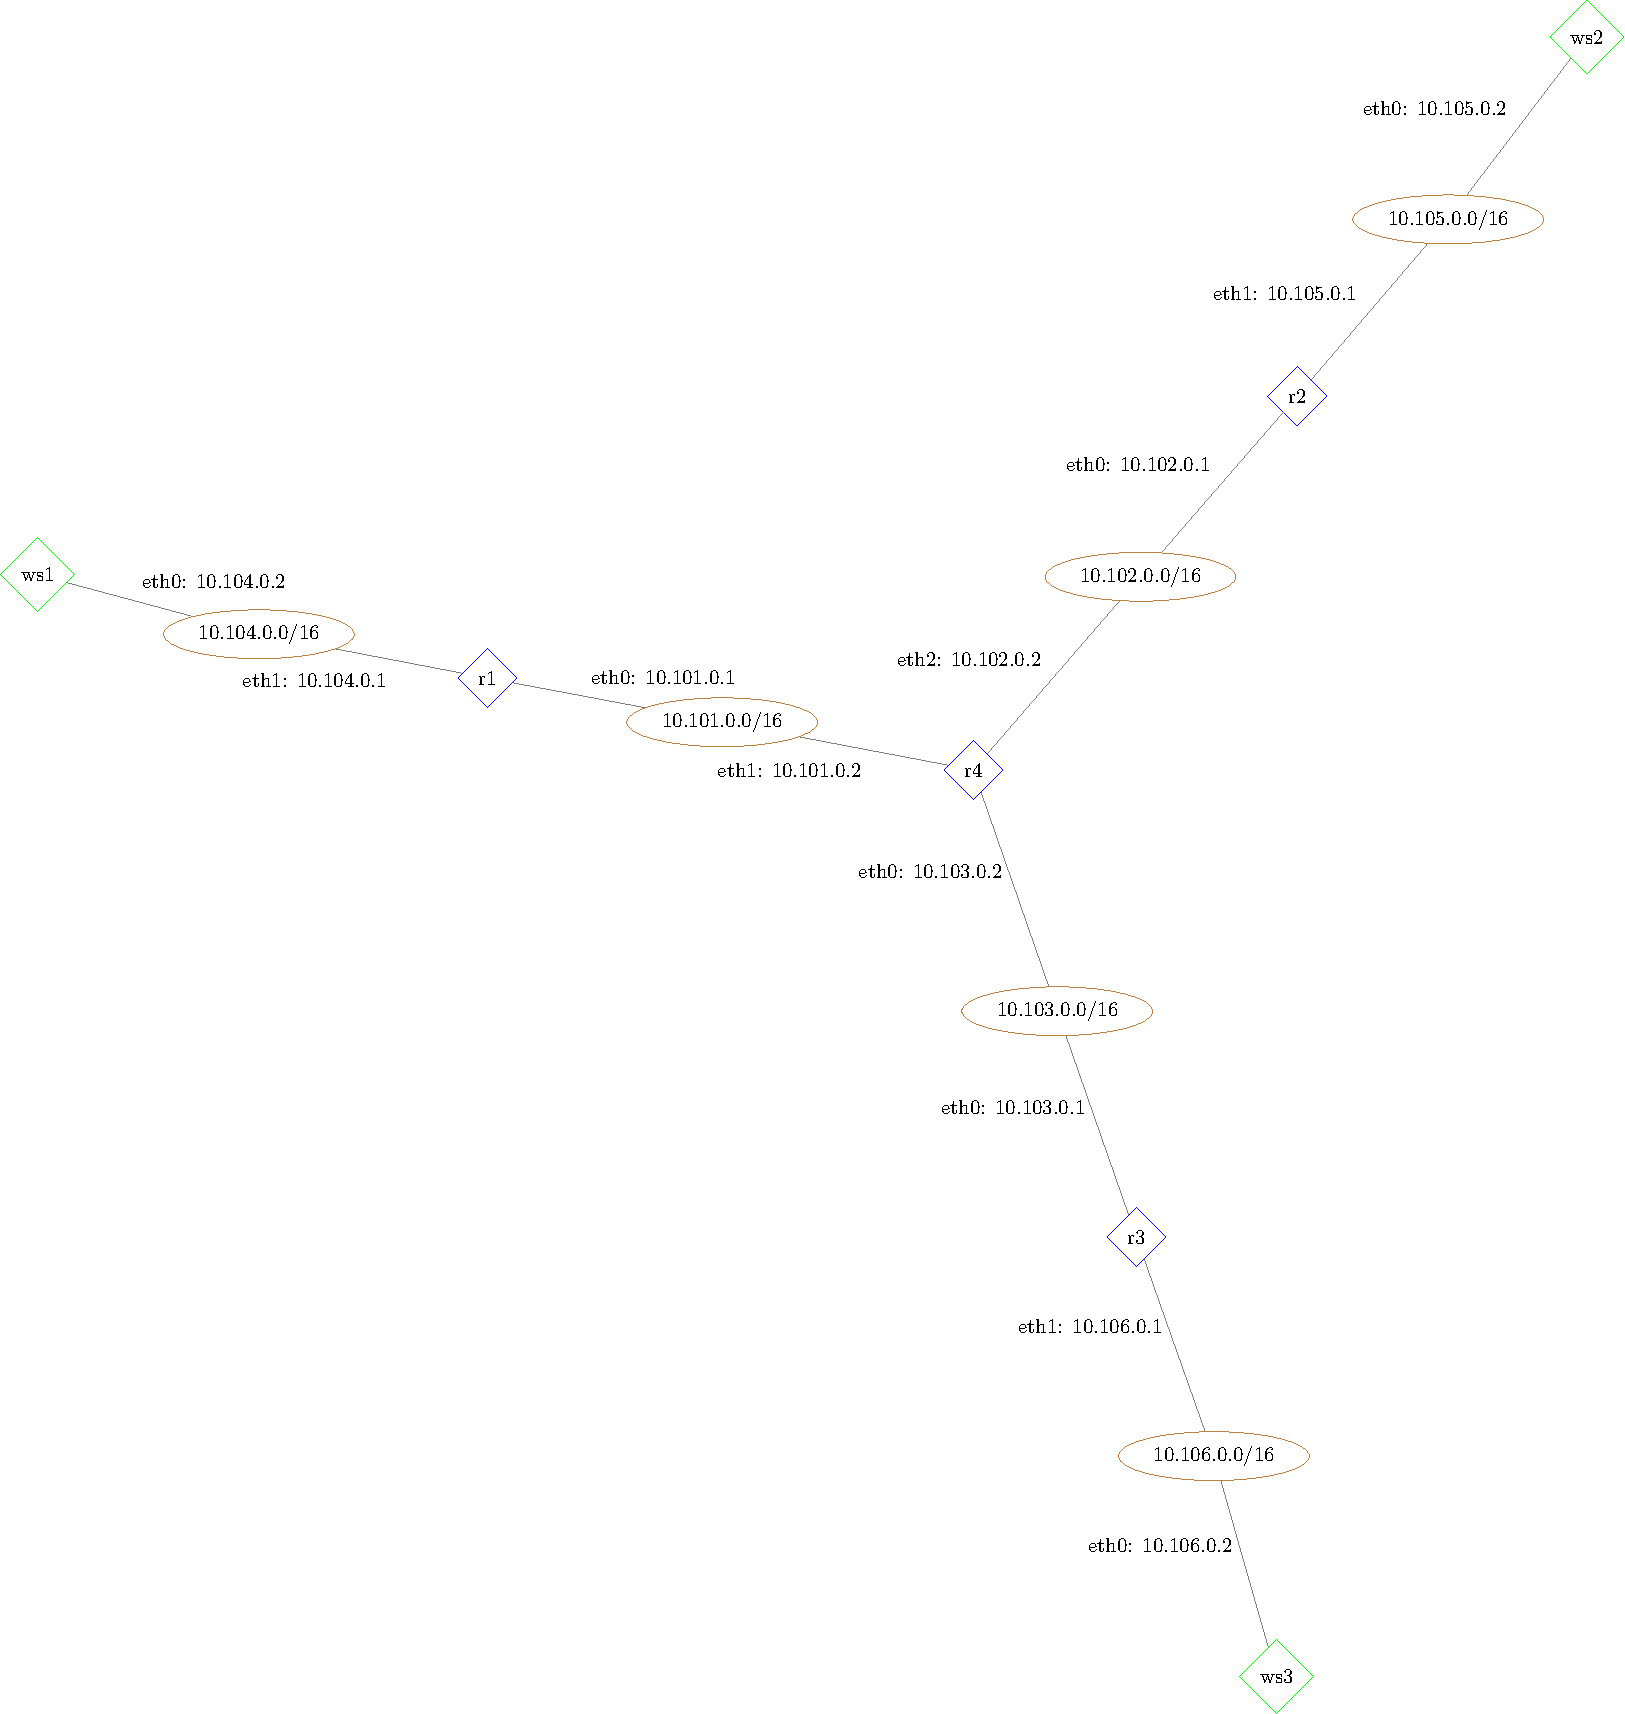
\includegraphics[width=\textwidth]{includes/network_gv.pdf}
\caption{Топология сети}
\label{fig:network}
\end{figure}


\section{Назначение IP-адресов}

Ниже приведён файл настройки протокола IP маршрутизатора r1.

\begin{Verbatim}
auto lo
iface lo inet loopback

auto eth0
iface eth0 inet static
address 10.101.0.1
netmask 255.255.0.0
up ip r add 10.103.0.0/16 via 10.101.0.2 dev eth0
up ip r add 10.106.0.0/16 via 10.101.0.2 dev eth0
up ip r add 10.102.0.0/16 via 10.101.0.2 dev eth0
up ip r add 10.105.0.0/16 via 10.101.0.2 dev eth0
down ip r del 10.103.0.0/16
down ip r del 10.106.0.0/16
down ip r del 10.102.0.0/16
down ip r del 10.105.0.0/16

auto eth1
iface eth1 inet static
address 10.104.0.1
netmask 255.255.0.0
\end{Verbatim}

Ниже приведён файл настройки протокола IP рабочей станции ws1.

\begin{Verbatim}
auto lo
iface lo inet loopback

auto eth0
iface eth0 inet static
address 10.104.0.2
netmask 255.255.0.0
gateway 10.104.0.1
\end{Verbatim}


\section{Таблица маршрутизации}

Таблица маршрутизации для \textbf{r1}.

\begin{Verbatim}
10.101.0.0/16 dev eth0  proto kernel  scope link  src 10.101.0.1 
10.103.0.0/16 via 10.101.0.2 dev eth0 
10.102.0.0/16 via 10.101.0.2 dev eth0 
10.105.0.0/16 via 10.101.0.2 dev eth0 
10.104.0.0/16 dev eth1  proto kernel  scope link  src 10.104.0.1 
10.106.0.0/16 via 10.101.0.2 dev eth0 
\end{Verbatim}

Таблица маршрутизации для \textbf{r2}.

\begin{Verbatim}
10.101.0.0/16 via 10.102.0.2 dev eth0 
10.103.0.0/16 via 10.102.0.2 dev eth0 
10.102.0.0/16 dev eth0  proto kernel  scope link  src 10.102.0.1 
10.105.0.0/16 dev eth1  proto kernel  scope link  src 10.105.0.1 
10.104.0.0/16 via 10.102.0.2 dev eth0 
10.106.0.0/16 via 10.102.0.2 dev eth0
\end{Verbatim}

Таблица маршрутизации для \textbf{r3}.

\begin{Verbatim}
10.101.0.0/16 via 10.103.0.2 dev eth0 
10.103.0.0/16 dev eth0  proto kernel  scope link  src 10.103.0.1 
10.102.0.0/16 via 10.103.0.2 dev eth0 
10.105.0.0/16 via 10.103.0.2 dev eth0 
10.104.0.0/16 via 10.103.0.2 dev eth0 
10.106.0.0/16 dev eth1  proto kernel  scope link  src 10.106.0.1 
\end{Verbatim}

Таблица маршрутизации для \textbf{r4}.

\begin{Verbatim}
10.101.0.0/16 dev eth1  proto kernel  scope link  src 10.101.0.2 
10.103.0.0/16 dev eth0  proto kernel  scope link  src 10.103.0.2 
10.102.0.0/16 dev eth2  proto kernel  scope link  src 10.102.0.2 
10.105.0.0/16 via 10.102.0.1 dev eth2 
10.104.0.0/16 via 10.101.0.1 dev eth1 
10.106.0.0/16 via 10.103.0.1 dev eth0 
\end{Verbatim}

% ... Повторять для всех маршрутизаторов и рабочих станций, где есть что-то кроме gateway.

\section{Проверка настройки сети}

Вывод \textbf{traceroute} от узла ws1 до ws2 при нормальной работе сети.

\begin{Verbatim}
ws1:~# traceroute -n 10.105.0.2
traceroute to 10.105.0.2 (10.105.0.2), 64 hops max, 40 byte packets
 1  10.104.0.1  2 ms  1 ms  0 ms
 2  10.101.0.2  0 ms  0 ms  0 ms
 3  10.102.0.1  10 ms  0 ms  0 ms
 4  10.105.0.2  12 ms  0 ms  0 ms
\end{Verbatim}

Вывод \textbf{traceroute} от узла ws1 до ws3 при нормальной работе сети.

\begin{Verbatim}
ws1:~# traceroute -n 10.106.0.2
traceroute to 10.106.0.2 (10.106.0.2), 64 hops max, 40 byte packets
 1  10.104.0.1  3 ms  0 ms  0 ms
 2  10.101.0.2  11 ms  0 ms  0 ms
 3  10.103.0.1  14 ms  0 ms  0 ms
 4  10.106.0.2  10 ms  0 ms  0 ms
\end{Verbatim}

Вывод \textbf{traceroute} от узла ws2 до ws3 при нормальной работе сети.

\begin{Verbatim}
ws2:~# traceroute -n 10.106.0.2
traceroute to 10.106.0.2 (10.106.0.2), 64 hops max, 40 byte packets
 1  10.105.0.1  0 ms  0 ms  0 ms
 2  10.102.0.2  0 ms  0 ms  0 ms
 3  10.103.0.1  11 ms  2 ms  1 ms
 4  10.106.0.2  11 ms  2 ms  1 ms
\end{Verbatim}


\section{Маршрутизация}

% На пути здесь достаточно быть одному аршрутизатору!

Опишем, какие MAC-адреса интерфейсов у каких машин.

\begin{Verbatim}
r1, eth0: 0e:ab:f8:0c:10:4b
r1, eth1: fa:de:dc:30:96:57

r2, eth0: 3a:40:ee:31:9e:cd
r2, eth1: 12:3e:e2:7d:e3:87

r3, eth0: ee:97:f2:ab:47:0c
r3, eth1: d2:90:43:d2:95:19

r4, eth0: 4a:e4:d9:3b:f2:04
r4, eth1: 42:9b:97:db:b0:a6
r4, eth2: 8e:49:ea:71:64:6b

ws1, eth0: a6:f9:52:b6:1e:69

ws2, eth0: da:53:12:09:ea:4e

ws3, eth0: b2:0b:69:d6:a7:1e
\end{Verbatim}

Выведем маршрутную таблицу маршрутизатора r1 (вывод команды ip r)

\begin{Verbatim}
10.101.0.0/16 dev eth0  proto kernel  scope link  src 10.101.0.1 
10.103.0.0/16 via 10.101.0.2 dev eth0 
10.102.0.0/16 via 10.101.0.2 dev eth0 
10.105.0.0/16 via 10.101.0.2 dev eth0 
10.104.0.0/16 dev eth1  proto kernel  scope link  src 10.104.0.1 
10.106.0.0/16 via 10.101.0.2 dev eth0 
\end{Verbatim}

Показаны опыты после стирания кеша ARP.
% Не забудьте это сделать!
Далее показана отправка пакета с рабочей станции ws3 на маршрутизатор r4 через r3(косвенная маршрутизация). 

\begin{Verbatim}
ws3:~# ping 10.103.0.2 -c 1
PING 10.103.0.2 (10.103.0.2) 56(84) bytes of data.
64 bytes from 10.103.0.2: icmp_seq=1 ttl=63 time=18.0 ms

--- 10.103.0.2 ping statistics ---
1 packets transmitted, 1 received, 0% packet loss, time 0ms
rtt min/avg/max/mdev = 18.073/18.073/18.073/0.000 ms

ws3:~# ip n
10.106.0.1 dev eth0 lladdr d2:90:43:d2:95:19 REACHABLE
\end{Verbatim}

Затем маршрутизатор отправил его далее.

\begin{Verbatim}
r3:~# tcpdump -ntve -i eth1
tcpdump: listening on eth1, link-type EN10MB (Ethernet), capture size 96 bytes
b2:0b:69:d6:a7:1e > ff:ff:ff:ff:ff:ff, ethertype ARP (0x0806), length 42: arp who-has 10.106.0.1 tell 10.106.0.2
d2:90:43:d2:95:19 > b2:0b:69:d6:a7:1e, ethertype ARP (0x0806), length 42: arp reply 10.106.0.1 is-at d2:90:43:d2:95:19
b2:0b:69:d6:a7:1e > d2:90:43:d2:95:19, ethertype IPv4 (0x0800), length 98: (tos 0x0, ttl 64, id 0, offset 0, flags [DF], proto ICMP (1), length 84) 10.106.0.2 > 10.103.0.2: ICMP echo request, id 12802, seq 1, length 64
d2:90:43:d2:95:19 > b2:0b:69:d6:a7:1e, ethertype IPv4 (0x0800), length 98: (tos 0x0, ttl 63, id 47698, offset 0, flags [none], proto ICMP (1), length 84) 10.103.0.2 > 10.106.0.2: ICMP echo reply, id 12802, seq 1, length 64
d2:90:43:d2:95:19 > b2:0b:69:d6:a7:1e, ethertype ARP (0x0806), length 42: arp who-has 10.106.0.2 tell 10.106.0.1
b2:0b:69:d6:a7:1e > d2:90:43:d2:95:19, ethertype ARP (0x0806), length 42: arp reply 10.106.0.2 is-at b2:0b:69:d6:a7:1e
^C
6 packets captured
\end{Verbatim}

И затем конечный получатель (маршрутизатор r4) получил сообщение.

\begin{Verbatim}
r4:~# tcpdump -ntve -i eth0
tcpdump: listening on eth0, link-type EN10MB (Ethernet), capture size 96 bytes
ee:97:f2:ab:47:0c > ff:ff:ff:ff:ff:ff, ethertype ARP (0x0806), length 42: arp who-has 10.103.0.2 tell 10.103.0.1
4a:e4:d9:3b:f2:04 > ee:97:f2:ab:47:0c, ethertype ARP (0x0806), length 42: arp reply 10.103.0.2 is-at 4a:e4:d9:3b:f2:04
ee:97:f2:ab:47:0c > 4a:e4:d9:3b:f2:04, ethertype IPv4 (0x0800), length 98: (tos 0x0, ttl 63, id 0, offset 0, flags [DF], proto ICMP (1), length 84) 10.106.0.2 > 10.103.0.2: ICMP echo request, id 12802, seq 1, length 64
4a:e4:d9:3b:f2:04 > ee:97:f2:ab:47:0c, ethertype IPv4 (0x0800), length 98: (tos 0x0, ttl 64, id 47698, offset 0, flags [none], proto ICMP (1), length 84) 10.103.0.2 > 10.106.0.2: ICMP echo reply, id 12802, seq 1, length 64
4a:e4:d9:3b:f2:04 > ee:97:f2:ab:47:0c, ethertype ARP (0x0806), length 42: arp who-has 10.103.0.1 tell 10.103.0.2
ee:97:f2:ab:47:0c > 4a:e4:d9:3b:f2:04, ethertype ARP (0x0806), length 42: arp reply 10.103.0.1 is-at ee:97:f2:ab:47:0c
^C
6 packets captured
\end{Verbatim}

\section{Продолжительность жизни пакета} 
Для опыта с продолжительностью жизни пакета (TTL), создадим маршрутную петлю между маршрутизаторами r1 и r4. 

\begin{Verbatim}
r4:~# ip link set eth2 down
r4:~# ip link set eth0 down
r4:~# ip l
1: lo: <LOOPBACK,UP,LOWER_UP> mtu 16436 qdisc noqueue 
    link/loopback 00:00:00:00:00:00 brd 00:00:00:00:00:00
2: teql0: <NOARP> mtu 1500 qdisc noop qlen 100
    link/void 
3: eth0: <BROADCAST,MULTICAST> mtu 1500 qdisc pfifo_fast qlen 1000
    link/ether 4a:e4:d9:3b:f2:04 brd ff:ff:ff:ff:ff:ff
4: eth1: <BROADCAST,MULTICAST,UP,LOWER_UP> mtu 1500 qdisc pfifo_fast qlen 1000
    link/ether 42:9b:97:db:b0:a6 brd ff:ff:ff:ff:ff:ff
5: eth2: <BROADCAST,MULTICAST> mtu 1500 qdisc pfifo_fast qlen 1000
    link/ether 8e:49:ea:71:64:6b brd ff:ff:ff:ff:ff:ff
r4:~# ip route add 10.103.0.0/16 via 10.101.0.1 dev eth1
\end{Verbatim}

Измененная таблица маршратизации для маршрутизатора r4 выглядит следующим образом.

\begin{Verbatim}
r4:~# ip r
10.101.0.0/16 dev eth1  proto kernel  scope link  src 10.101.0.2 
10.103.0.0/16 via 10.101.0.1 dev eth1 
10.104.0.0/16 via 10.101.0.1 dev eth1 
\end{Verbatim}

Отправляем сообщение с рабочей станции ws1 на маршрутизатор r3 .

\begin{Verbatim}
ws1:~# ping 10.103.0.1 -c 1
PING 10.103.0.1 (10.103.0.1) 56(84) bytes of data.
From 10.101.0.2 icmp_seq=1 Time to live exceeded

--- 10.103.0.1 ping statistics ---
1 packets transmitted, 0 received, +1 errors, 100% packet loss, time 0ms
\end{Verbatim}

Получаем ICMP сообщение об истечении TTL отправленного сообщения.
На маршрутизаторе r1 происходит отправка сообщений маршрутизатору r4 и циклическая отправка в маршрутной петле.

\begin{Verbatim}
r1:~# tcpdump -ntve -i any
tcpdump: listening on any, link-type LINUX_SLL (Linux cooked), capture size 96 bytes
  B a6:f9:52:b6:1e:69 ethertype ARP (0x0806), length 44: arp who-has 10.104.0.1 tell 10.104.0.2
Out fa:de:dc:30:96:57 ethertype ARP (0x0806), length 44: arp reply 10.104.0.1 is-at fa:de:dc:30:96:57
 In a6:f9:52:b6:1e:69 ethertype IPv4 (0x0800), length 100: (tos 0x0, ttl 64, id 0, offset 0, flags [DF], proto ICMP (1), length 84) 10.104.0.2 > 10.103.0.1: ICMP echo request, id 13826, seq 1, length 64
Out 0e:ab:f8:0c:10:4b ethertype ARP (0x0806), length 44: arp who-has 10.101.0.2 tell 10.101.0.1
 In 42:9b:97:db:b0:a6 ethertype ARP (0x0806), length 44: arp reply 10.101.0.2 is-at 42:9b:97:db:b0:a6
Out 0e:ab:f8:0c:10:4b ethertype IPv4 (0x0800), length 100: (tos 0x0, ttl 63, id 0, offset 0, flags [DF], proto ICMP (1), length 84) 10.104.0.2 > 10.103.0.1: ICMP echo request, id 13826, seq 1, length 64
 In 42:9b:97:db:b0:a6 ethertype IPv4 (0x0800), length 100: (tos 0x0, ttl 62, id 0, offset 0, flags [DF], proto ICMP (1), length 84) 10.104.0.2 > 10.103.0.1: ICMP echo request, id 13826, seq 1, length 64


...


Out 0e:ab:f8:0c:10:4b ethertype IPv4 (0x0800), length 100: (tos 0x0, ttl 1, id 0, offset 0, flags [DF], proto ICMP (1), length 84) 10.104.0.2 > 10.103.0.1: ICMP echo request, id 13826, seq 1, length 64
 In 42:9b:97:db:b0:a6 ethertype IPv4 (0x0800), length 128: (tos 0xc0, ttl 64, id 5356, offset 0, flags [none], proto ICMP (1), length 112) 10.101.0.2 > 10.104.0.2: ICMP time exceeded in-transit, length 92
	(tos 0x0, ttl 1, id 0, offset 0, flags [DF], proto ICMP (1), length 84) 10.104.0.2 > 10.103.0.1: ICMP echo request, id 13826, seq 1, length 64
Out fa:de:dc:30:96:57 ethertype IPv4 (0x0800), length 128: (tos 0xc0, ttl 63, id 5356, offset 0, flags [none], proto ICMP (1), length 112) 10.101.0.2 > 10.104.0.2: ICMP time exceeded in-transit, length 92
	(tos 0x0, ttl 1, id 0, offset 0, flags [DF], proto ICMP (1), length 84) 10.104.0.2 > 10.103.0.1: ICMP echo request, id 13826, seq 1, length 64

\end{Verbatim}

Итоговое ICMP сообщение об истечении TTL было отправлено маршрутизатором r4, что видно из IP адреса отправителя сообщения.

\section{Изучение IP-фрагментации}

Изменяем значение MTU в сети 10.101.0.0/16 (т.е. изменяем значение на сетевых интерфейсах eth0 маршрутизатора r1 и eth1 маршрутизатора r4. 

\begin{Verbatim}
r1:~# ip link set dev eth0 mtu 576
\end{Verbatim}

\begin{Verbatim}
r4:~# ip link set dev eth1 mtu 576
\end{Verbatim}

% Напоминаем, что PMTU следует отключить!

Отключаем параметр PMTU и используем команду ping для тестирования.

\begin{Verbatim}
ws1:~# echo 1 > /proc/sys/net/ipv4/ip_no_pmtu_disc
ws1:~# ping -c 1 -s 1000 10.103.0.1
PING 10.103.0.1 (10.103.0.1) 1000(1028) bytes of data.
1008 bytes from 10.103.0.1: icmp_seq=1 ttl=62 time=2.78 ms

--- 10.103.0.1 ping statistics ---
1 packets transmitted, 1 received, 0% packet loss, time 0ms
rtt min/avg/max/mdev = 2.780/2.780/2.780/0.000 ms
\end{Verbatim}

Вывод \textbf{tcpdump} на маршрутизаторе перед сетью с уменьшенным MTU.

% Вывод в ширину можно и сократить, удалив несущественные моменты!

\begin{Verbatim}
r1:~# tcpdump -tnv -i eth1 icmp
tcpdump: listening on eth1, link-type EN10MB (Ethernet), capture size 96 bytes
IP (tos 0x0, ttl 64, id 11922, offset 0, flags [none], proto ICMP (1), length 1028) 10.104.0.2 > 10.103.0.1: ICMP echo request, id 18946, seq 1, length 1008
IP (tos 0x0, ttl 62, id 59858, offset 0, flags [none], proto ICMP (1), length 1028) 10.103.0.1 > 10.104.0.2: ICMP echo reply, id 18946, seq 1, length 1008
\end{Verbatim}

Вывод \textbf{tcpdump} на маршрутизаторе после сети с уменьшенным MTU.

% Вывод в ширину можно и сократить, удалив несущественные моменты!

\begin{Verbatim}
r4:~#  tcpdump -tnv -i eth1 icmp
tcpdump: listening on eth1, link-type EN10MB (Ethernet), capture size 96 bytes
IP (tos 0x0, ttl 63, id 11922, offset 0, flags [+], proto ICMP (1), length 572) 10.104.0.2 > 10.103.0.1: ICMP echo request, id 18946, seq 1, length 552
IP (tos 0x0, ttl 63, id 11922, offset 552, flags [none], proto ICMP (1), length 476) 10.104.0.2 > 10.103.0.1: icmp
IP (tos 0x0, ttl 63, id 59858, offset 0, flags [+], proto ICMP (1), length 572) 10.103.0.1 > 10.104.0.2: ICMP echo reply, id 18946, seq 1, length 552
IP (tos 0x0, ttl 63, id 59858, offset 552, flags [none], proto ICMP (1), length 476) 10.103.0.1 > 10.104.0.2: icmp
\end{Verbatim}


Вывод \textbf{tcpdump} на узле получателя.

\begin{Verbatim}
r3:~#  tcpdump -tnv -i eth0 icmp
tcpdump: listening on eth0, link-type EN10MB (Ethernet), capture size 96 bytes
IP (tos 0x0, ttl 62, id 11922, offset 0, flags [none], proto ICMP (1), length 1028) 10.104.0.2 > 10.103.0.1: ICMP echo request, id 18946, seq 1, length 1008
IP (tos 0x0, ttl 64, id 59858, offset 0, flags [none], proto ICMP (1), length 1028) 10.103.0.1 > 10.104.0.2: ICMP echo reply, id 18946, seq 1, length 1008
\end{Verbatim}


\section{Отсутствие сети}

Проведем опыт с отуствием получателя в таблице маршрутизатора. Запустим перехват сообщений на маршрутизатора r1 и отправим сообщение с рабочей станции 1 на адрес с несуществующей сетью.

\begin{Verbatim}
ws1:~# ping -c 1 10.110.0.1
PING 10.110.0.1 (10.110.0.1) 56(84) bytes of data.
From 10.104.0.1 icmp_seq=1 Destination Net Unreachable

--- 10.110.0.1 ping statistics ---
1 packets transmitted, 0 received, +1 errors, 100% packet loss, time 0ms

r1:~# tcpdump -n -i eth1 icmp
tcpdump: verbose output suppressed, use -v or -vv for full protocol decode
listening on eth1, link-type EN10MB (Ethernet), capture size 96 bytes
10:24:52.151525 IP 10.104.0.2 > 10.110.0.1: ICMP echo request, id 19202, seq 1, length 64
10:24:52.151545 IP 10.104.0.1 > 10.104.0.2: ICMP net 10.110.0.1 unreachable, length 92
\end{Verbatim}


\section{Отсутствие IP-адреса в сети}

Проведем опыт с отсутствием получателя в сегменте сети. Запустим перехват сообщений на маршрутизаторе r1 и отправим сообщение с рабочей станции 1 на несуществующий адрес.

\begin{Verbatim}
ws1:~# ping -c 1 10.101.0.5
PING 10.101.0.5 (10.101.0.5) 56(84) bytes of data.
From 10.104.0.1 icmp_seq=1 Destination Host Unreachable

--- 10.101.0.5 ping statistics ---
1 packets transmitted, 0 received, +1 errors, 100% packet loss, time 0ms


r1:~# tcpdump -n -i eth1
tcpdump: verbose output suppressed, use -v or -vv for full protocol decode
listening on eth1, link-type EN10MB (Ethernet), capture size 96 bytes
10:29:37.165939 IP 10.104.0.2 > 10.101.0.5: ICMP echo request, id 19458, seq 1, length 64
10:29:40.185390 IP 10.104.0.1 > 10.104.0.2: ICMP host 10.101.0.5 unreachable, length 92
10:29:42.155319 arp who-has 10.104.0.1 tell 10.104.0.2
10:29:42.155329 arp reply 10.104.0.1 is-at fa:de:dc:30:96:57

\end{Verbatim}

\end{document}
